\chapter{Applicazioni di elaborazioni omomorfiche a scenari medicali}

\section{Introduzione}
In questo capitolo si considera un'applicazione concreta: l'uso della regressione lineare in uno scenario medico. L'idea di fondo \`e semplice. Pi\`u strutture sanitarie o pi\`u soggetti che raccolgono dati clinici vogliono contribuire alla costruzione di un modello statistico, ma senza rinunciare alla protezione delle informazioni trattate.

Nel caso concreto considerato, la regressione lineare viene usata per stimare il numero di giorni di permanenza in ospedale di un paziente a partire da et\`a, indice di comorbilit\`a di Charlson, numero di procedure precedenti, pressione sistolica e diastolica e indice di massa corporea. Il capitolo mostra come questo modello venga inserito in un'architettura i cui attori principali sono:
\begin{itemize}
  \item il \emph{setup authority}, che crea il contesto crittografico e genera le chiavi del sistema;
  \item il \emph{data provider}, che possiede i dati clinici originari;
  \item il \emph{computation server}, che esegue il training del modello o le valutazioni numeriche;
  \item il \emph{query actor}, che desidera interrogare il modello;
  \item il \emph{decryptor}, che pu\`o coincidere con un soggetto istituzionale, ad esempio il SSN, e che detiene la capacit\`a di decifrare i risultati.
\end{itemize}

La separazione tra computation server e decryptor \`e intenzionale. Le computazioni omomorfiche possono richiedere tempi elevati e possono quindi essere affidate anche a soggetti terzi specializzati, senza esporre in chiaro i dati sensibili o le query dei pazienti. Il decryptor resta invece il soggetto che possiede la chiave segreta e rende leggibile solo il risultato finale. A monte, il setup authority inizializza il sistema e distribuisce chiave pubblica, chiave segreta ed eventuali evaluation keys agli attori autorizzati.

Nel primo scenario il query actor invia query cifrate al computation server e riceve un risultato cifrato, poi decifrato dal decryptor. Nel secondo il computation server invia il polinomio cifrato al decryptor, mentre il query actor interroga in chiaro il servizio del soggetto fiduciario.

\section{Richiami sulla regressione lineare}
La regressione lineare serve a trovare una relazione semplice tra dati in ingresso e dato in uscita. In altre parole, si parte da esempi gi\`a osservati e si cerca una formula che descriva il loro andamento medio.

Il dataset contiene pi\`u osservazioni, una per ciascun paziente. Ogni osservazione comprende sei valori di ingresso: et\`a, indice di comorbilit\`a di Charlson, numero di procedure precedenti, pressione sistolica, pressione diastolica e indice di massa corporea. A questi sei valori corrisponde un unico valore da prevedere, cio\`e il numero di giorni di permanenza in ospedale.

Nel caso con pi\`u variabili in ingresso, il modello si scrive come
\begin{equation}
\hat{y} = w^T x + b = \sum_{j=1}^{6} w_j x_j + b,
\end{equation}
dove:
\begin{itemize}
  \item $w$ contiene i coefficienti del modello;
  \item $x$ contiene i sei valori di ingresso relativi al paziente;
  \item $b$ \`e il bias;
  \item $\hat{y}$ \`e il numero stimato di giorni di permanenza in ospedale.
\end{itemize}

La regressione adottata \`e lineare perch\'e tutte le variabili $x_j$ compaiono esclusivamente alla prima potenza: il modello non contiene termini quadratici, potenze superiori o interazioni tra feature. Questa scelta costituisce una semplificazione intenzionale. Variabili come la pressione sistolica e diastolica possono infatti avere una relazione pi\`u complessa e non lineare con la durata del ricovero; in un'applicazione clinica completa si potrebbero quindi considerare trasformazioni delle feature o modelli differenti. Nel presente caso si mantiene invece una funzione affine di primo grado, poich\'e lo scopo principale \`e dimostrare in modo semplice e leggibile l'applicazione delle tecniche omomorfiche.

\subsection{Funzione di costo}
Per capire se la retta trovata \`e buona oppure no, bisogna confrontare le previsioni del modello con i valori reali. Durante l'ottimizzazione si considera la met\`a dell'errore quadratico medio:
\begin{equation}
J(w,b) = \frac{1}{2n}\sum_{i=1}^{n}(\hat{y}_i - y_i)^2.
\end{equation}
Il fattore $1/2$ semplifica il calcolo del gradiente e non cambia i valori di $w$ e $b$ che minimizzano la funzione. La MSE completa, pari a $2J(w,b)$, viene usata per monitorare l'andamento del training. Se $J(w,b)$ \`e piccolo, il modello rappresenta bene le osservazioni disponibili.

\subsection{Determinazione dei coefficienti}
I coefficienti non vengono ricavati calcolando direttamente l'inversa di una matrice. Il modello usa invece la \emph{discesa del gradiente} (\emph{gradient descent}), un procedimento iterativo che parte da coefficienti iniziali molto semplici e li corregge poco alla volta nella direzione che riduce la funzione di costo.

Il training parte da pesi e bias nulli e, per un numero prefissato di epoche, calcola la previsione, misura l'errore e aggiorna i coefficienti usando un learning rate $\eta$.

In forma compatta, la previsione del modello \`e
\begin{equation}
\hat{y} = Xw + b\mathbf{1}_n,
\end{equation}
 dove $\mathbf{1}_n$ \`e un vettore di $n$ elementi uguali a uno e indica che lo stesso bias viene aggiunto alla previsione di ogni paziente.
Successivamente si calcola il vettore degli errori:
\begin{equation}
E = \hat{y} - y.
\end{equation}
Se una previsione \`e troppo alta rispetto al valore reale, l'errore sar\`a positivo; se invece \`e troppo bassa, l'errore sar\`a negativo.

Una volta ottenuto l'errore, il modello aggiorna i pesi tramite
\begin{equation}
w \leftarrow w - \eta \frac{1}{n} X^T E
\end{equation}
e aggiorna il bias tramite
\begin{equation}
b \leftarrow b - \eta \cdot \frac{1}{n}\sum_{i=1}^{n} E_i.
\end{equation}

Se il modello sbaglia sistematicamente in una direzione, i coefficienti vengono spostati gradualmente nella direzione opposta. La MSE viene calcolata a ogni epoca per verificare il miglioramento.

\subsection{Interpretazione in ambito medico}
Nel caso considerato, il modello assume la forma
\begin{equation}
\hat{y}=w_1\,\text{age}+w_2\,\text{cci}
+w_3\,\text{num\_procedures}+w_4\,\text{systolic}
+w_5\,\text{diastolic}+w_6\,\text{bmi}+b,
\end{equation}
dove $\hat{y}$ \`e la permanenza stimata in ospedale, espressa in giorni. I coefficienti descrivono il contributo delle singole feature:
\begin{itemize}
  \item $w_1$ \`e associato all'et\`a del paziente, compresa nell'intervallo $[0,100]$ anni;
  \item $w_2$ \`e associato al Charlson Comorbidity Index, compreso nell'intervallo $[0,37]$;
  \item $w_3$ \`e associato al numero di procedure o interventi precedenti, compreso nell'intervallo $[0,20]$;
  \item $w_4$ \`e associato alla pressione sistolica, compresa nell'intervallo $[80,200]$ mmHg;
  \item $w_5$ \`e associato alla pressione diastolica, compresa nell'intervallo $[50,120]$ mmHg;
  \item $w_6$ \`e associato all'indice di massa corporea, compreso indicativamente nell'intervallo $[15,40]$;
  \item $b$ rappresenta il bias del modello.
\end{itemize}

Questi intervalli descrivono i valori attesi delle variabili di ingresso, non i possibili valori dei coefficienti appresi. Inoltre, i coefficienti esprimono associazioni apprese dal dataset e non relazioni causali.

\section{Regressione lineare ed elaborazione omomorfica}
Una volta costruito il modello, il passaggio successivo consiste nel capire come usarlo nei due scenari considerati. La regressione lineare si presta bene a questo contesto perch\'e, una volta noti i coefficienti, la previsione si ottiene con un calcolo molto semplice:
\begin{equation}
\hat{y} = w^T x + b = \sum_{j=1}^{d} w_j x_j + b.
\end{equation}
In sostanza, bisogna fare prodotti e somme. Questo rende il modello adatto a un uso pratico anche in un'architettura protetta, perch\'e la fase di inferenza non richiede logiche troppo complicate.

L'implementazione in FHE usa lo schema CKKS. Questa scelta \`e utile perch\'e consente di rappresentare ed elaborare anche valori non interi, caratteristica importante in regressione lineare quando coefficienti, medie o risultati intermedi non sono interi. Inoltre, nell'implementazione si ricorre al \emph{bootstrapping} per riazzerare la profondit\`a moltiplicativa del ciphertext, poich\'e durante la regressione lineare, in particolare nelle fasi iterative di calcolo, si accumulano molte moltiplicazioni omomorfiche. CKKS introduce approssimazioni numeriche e quindi piccoli errori di arrotondamento, ma nel contesto considerato tali differenze sono trascurabili ai fini del risultato finale.

Nel calcolo in chiaro si pu\`o pensare a $x$, $w$ ed $y$ come a vettori e matrici ordinarie. In FHE, invece, questi dati devono essere inseriti negli slot di un ciphertext. Per questo motivo l'implementazione non lavora direttamente con la matrice nella sua forma pi\`u intuitiva, ma la riorganizza in blocchi che possano essere sommati e ruotati in modo efficiente.

Nel presente contesto si pu\`o scomporre il problema in due fasi:
\begin{enumerate}
  \item \textbf{training del modello}: il computation server riceve i dati dai provider e costruisce i coefficienti della regressione;
  \item \textbf{inferenza o query}: un attore interroga il modello per ottenere una previsione su un nuovo input.
\end{enumerate}

Il punto interessante \`e che nei due scenari cambia soprattutto la fase di query. Il modello matematico resta lo stesso, ma cambia chi vede i dati in chiaro, chi esegue la valutazione finale e chi possiede le chiavi necessarie per decifrare.

\section{Scenario 1: query cifrata al computation server}
Nel primo scenario, il data provider invia i dati al computation server, che esegue la regressione lineare e costruisce il polinomio del modello. Successivamente, il query actor non invia un input in chiaro, ma una query cifrata. Il computation server valuta il modello sul dato cifrato e restituisce un risultato anch'esso cifrato. Infine, il query actor si rivolge a un servizio di decrypt, che pu\`o essere incarnato dal SSN, per ottenere il valore in chiaro.

\subsection{Schema logico}
Lo schema pu\`o essere rappresentato come segue, assumendo che il setup authority distribuisca preventivamente le chiavi ai vari attori autorizzati:
\begin{align}
&\text{Data Provider}_i \longrightarrow \text{Computation Server}: \mathsf{Enc}_{pk}(\text{record di training}_i), \\
&\text{Computation Server}: \text{training su dati cifrati e costruzione di } \mathsf{Enc}_{pk}(w,b), \\
&\text{Query Actor} \longrightarrow \text{Computation Server}: \mathsf{Enc}_{pk}(x_q), \\
&\text{Computation Server}: \text{valutazione del modello su } \mathsf{Enc}_{pk}(x_q), \\
&\text{Computation Server} \longrightarrow \text{Query Actor}: \mathsf{Enc}_{pk}(w^T x_q + b), \\
&\text{Query Actor} \longrightarrow \text{Decryptor/SSN}: \mathsf{Enc}_{pk}(w^T x_q + b), \\
&\text{Decryptor/SSN}: \mathsf{Dec}_{sk}\big(\mathsf{Enc}_{pk}(w^T x_q + b)\big), \\
&\text{Decryptor/SSN} \longrightarrow \text{Query Actor}: w^T x_q + b.
\end{align}

Il computation server addestra il modello e valuta il polinomio su query cifrate; il query actor vede il risultato in chiaro solo dopo l'intervento del decryptor.

\begin{figure}[H]
\centering
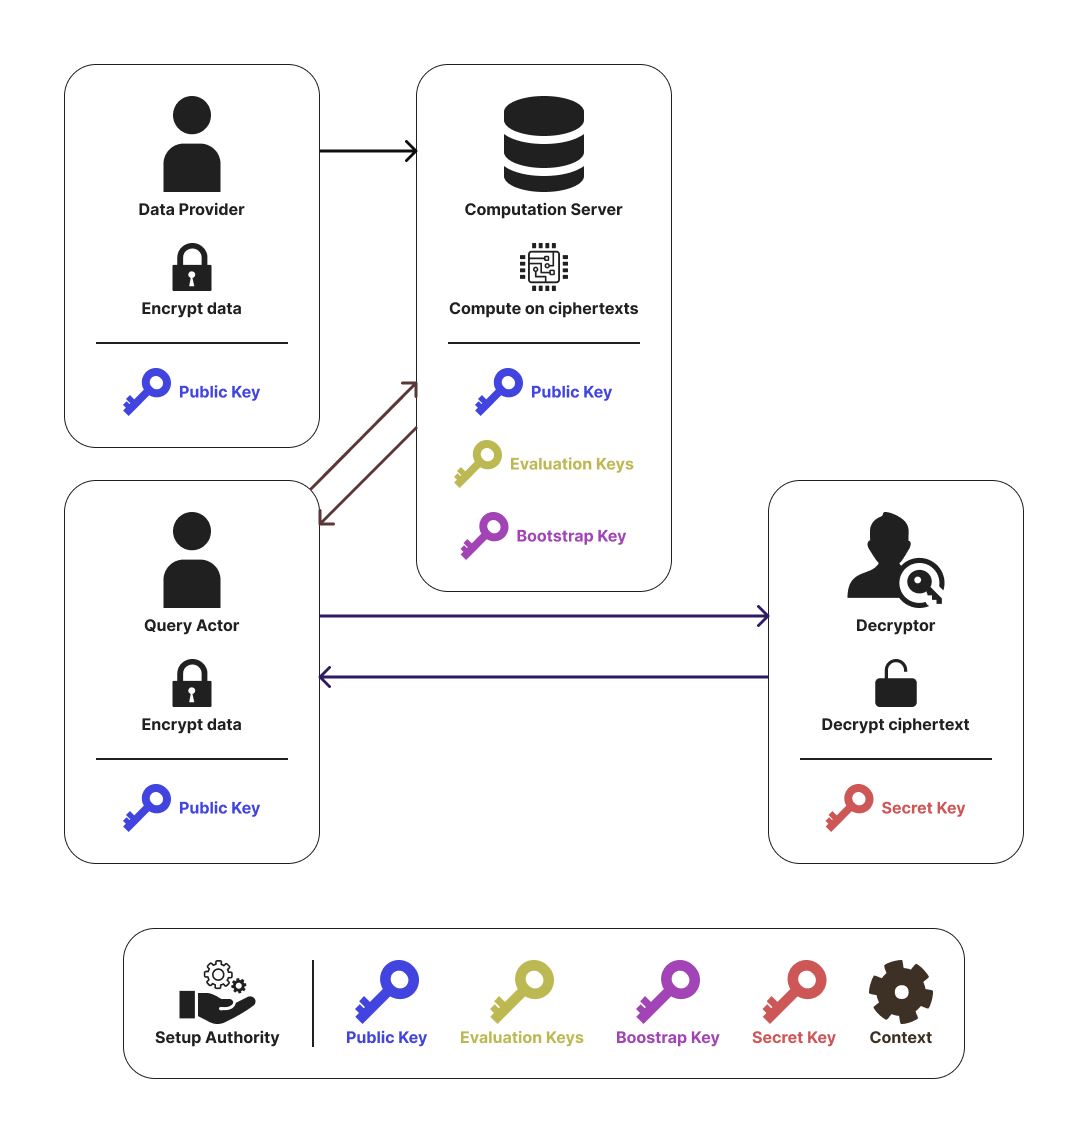
\includegraphics[width=0.95\textwidth]{figures/linear_regression_1.png}
\caption{Schema dello scenario 1.}
\label{fig:linear_regression_1}
\end{figure}

\subsection{Distribuzione delle chiavi}
In questo scenario si assume tipicamente la seguente ripartizione:
\begin{itemize}
  \item il \textbf{setup authority} genera il contesto crittografico, la chiave pubblica $pk$, la chiave segreta $sk$ ed eventuali evaluation keys, poi distribuisce tale materiale ai ruoli autorizzati;
  \item i \textbf{data provider} inviano al computation server soltanto dati cifrati con $pk$;
  \item il \textbf{computation server} conosce la chiave pubblica $pk$ e le eventuali evaluation keys necessarie alle operazioni omomorfiche;
  \item il \textbf{query actor} possiede o riceve la chiave pubblica $pk$ per cifrare le query;
  \item il \textbf{decryptor/SSN} possiede la chiave segreta $sk$;
\end{itemize}

La propriet\`a essenziale \`e che il computation server non dispone di $sk$, dunque non pu\`o vedere il contenuto delle query finali n\'e dei risultati cifrati che produce.

Lo scenario protegge la query e separa chi calcola da chi decifra. Richiede per\`o cifratura lato utente, gestione delle evaluation keys e l'intervento del decryptor, con maggiore complessit\`a e latenza.

\section{Scenario 2: il polinomio cifrato viene trasferito al decryptor}
Nel secondo scenario, il data provider invia i dati al computation server, che esegue il training del modello. Una volta ottenuti i coefficienti della regressione, il computation server cifra il polinomio e lo trasferisce direttamente al decryptor, ad esempio il SSN. Da quel momento, il query actor non interagisce pi\`u con il computation server per la fase di inferenza, ma invia le proprie query in chiaro al soggetto fiduciario.

\subsection{Schema logico}
Lo schema pu\`o essere espresso come segue, assumendo che il setup authority distribuisca preventivamente le chiavi ai vari attori autorizzati:
\begin{align}
&\text{Data Provider}_i \longrightarrow \text{Computation Server}: \mathsf{Enc}_{pk}(\text{record di training}_i), \\
&\text{Computation Server}: \text{training su dati cifrati e costruzione di } \mathsf{Enc}_{pk}(w,b), \\
&\text{Computation Server} \longrightarrow \text{Decryptor/SSN}: \mathsf{Enc}_{pk}(w,b), \\
&\text{Decryptor/SSN}: \mathsf{Dec}_{sk}\big(\mathsf{Enc}_{pk}(w,b)\big), \\
&\text{Query Actor} \longrightarrow \text{Decryptor/SSN}: x_q \text{ in chiaro}, \\
&\text{Decryptor/SSN} \longrightarrow \text{Query Actor}: w^T x_q + b.
\end{align}

Il query actor beneficia di un'interfaccia pi\`u semplice: non cifra nulla, ma si appoggia a un'entit\`a trusted che custodisce il modello e produce le risposte.

\begin{figure}[H]
\centering
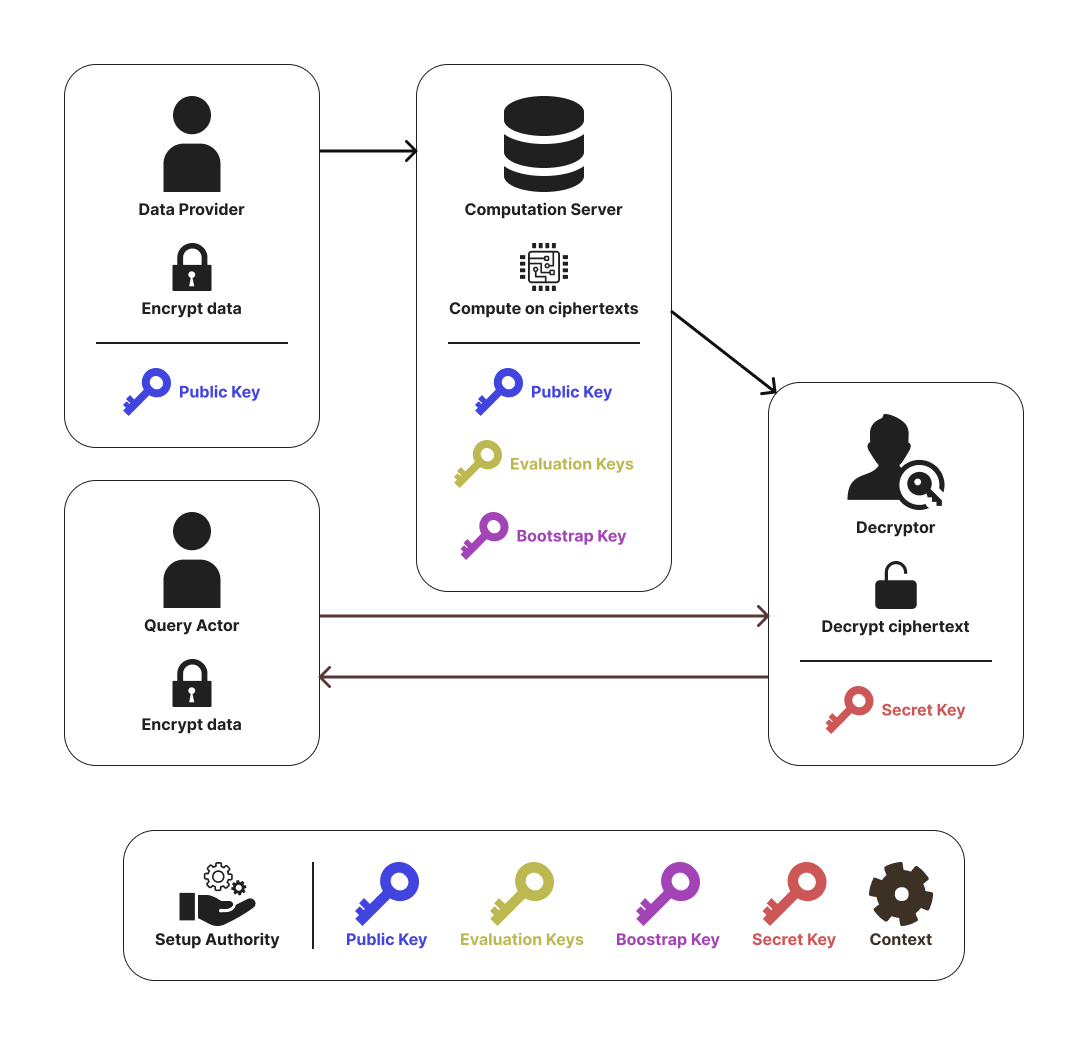
\includegraphics[width=0.95\textwidth]{figures/linear_regression_2.png}
\caption{Schema dello scenario 2.}
\label{fig:linear_regression_2}
\end{figure}

\subsection{Distribuzione delle chiavi}
La distribuzione delle chiavi \`e pi\`u centralizzata:
\begin{itemize}
  \item il \textbf{setup authority} genera il contesto crittografico, la chiave pubblica $pk$, la chiave segreta $sk$ ed eventuali evaluation keys, poi le distribuisce agli attori autorizzati;
  \item i \textbf{data provider} inviano al computation server soltanto dati cifrati con $pk$;
  \item il \textbf{computation server} conosce la chiave pubblica $pk$ e le eventuali evaluation keys necessarie alle operazioni omomorfiche;
  \item il \textbf{query actor} non ha bisogno di utilizzare direttamente chiavi crittografiche nella fase di interrogazione;
  \item il \textbf{decryptor/SSN} possiede la chiave segreta $sk$;
\end{itemize}

Questa architettura \`e coerente con contesti in cui il decryptor rappresenta un ente istituzionale gi\`a riconosciuto come fiduciario, in grado di custodire chiavi, modelli e risultati.

Lo scenario semplifica l'interrogazione e riduce la latenza, ma espone l'input al decryptor e concentra informazioni e fiducia presso tale ente. \`E quindi adatto quando la fiducia nel soggetto istituzionale \`e alta.

\section{Confronto tra le due architetture}
Le due architetture risolvono lo stesso problema, ma ottimizzano aspetti diversi. Una sintesi comparativa pu\`o essere espressa nella Tabella~\ref{tab:confronto_scenari}.

\begin{table}[h]
\centering
\begin{tabular}{|p{3.3cm}|p{5.2cm}|p{5.2cm}|}
\hline
\textbf{Aspetto} & \textbf{Scenario 1} & \textbf{Scenario 2} \\
\hline
Protezione delle query & Alta: il computation server riceve query cifrate & Pi\`u bassa: il query actor invia la query in chiaro al decryptor/SSN \\
\hline
Ruolo del computation server & Addestra il modello e valuta query cifrate & Addestra il modello e invia il polinomio cifrato al decryptor \\
\hline
Ruolo del decryptor & Decifra il risultato finale & Custodisce il modello e risponde alle query \\
\hline
Chiave segreta & Presso il decryptor/SSN & Presso il decryptor/SSN \\
\hline
Chiave pubblica & Usata da query actor e computation server & Usata da data provider e computation server \\
\hline
Complessit\`a per l'utente finale & Maggiore: deve cifrare la query & Minore: usa un'interfaccia in chiaro \\
\hline
Latenza complessiva & Pi\`u elevata & Pi\`u contenuta, ma con costo di inferenza a carico del decryptor/SSN \\
\hline
\end{tabular}
\caption{Confronto tra i due scenari di impiego della regressione lineare in ambito omomorfico-medicale.}
\label{tab:confronto_scenari}
\end{table}

Da questa tabella emerge un trade-off classico. Se si vuole proteggere fortemente la riservatezza dell'input di inferenza, lo scenario 1 \`e generalmente preferibile. Se invece si desidera un servizio pi\`u semplice, controllato da un ente sanitario centrale e pi\`u immediato da usare, lo scenario 2 pu\`o risultare pi\`u naturale. Va per\`o ricordato che, nello scenario 2, il training resta a carico del computation server mentre l'inferenza viene eseguita dal decryptor, cio\`e dal SSN: anche questa fase ha quindi un costo computazionale e operativo che deve essere sostenuto dall'attore ultimo invece del server computazionale che però essendo in chiaro risultat molto meno dispendioso del eseguire una decrifrazione.

\section{Esempio applicativo: stima dei giorni di ricovero}
Il dataset sanitario contiene, per ogni osservazione, le sei caratteristiche del paziente e il numero di giorni di permanenza in ospedale da apprendere. Alcune osservazioni sono:
\begin{center}
\begin{tabular}{|c|c|c|c|c|c|c|}
\hline
\textbf{Et\`a} & \textbf{CCI} & \textbf{Proc.} & \textbf{Sist.} &
\textbf{Diast.} & \textbf{BMI} & \textbf{Giorni} \\
\hline
37 & 2 & 12 & 148 & 106 & 22.5 & 4 \\
77 & 1 & 7 & 105 & 106 & 38.0 & 3 \\
83 & 2 & 17 & 82 & 64 & 29.2 & 5 \\
\hline
\end{tabular}
\end{center}

Il modello deve trovare i sei pesi e il bias che minimizzano l'errore tra i giorni stimati e quelli presenti nell'ultima colonna.

\subsection{Come parte il training}
Il training parte da coefficienti iniziali nulli:
\begin{equation}
w_1 = \cdots = w_6 = 0,
\qquad
b = 0.
\end{equation}

Con questa scelta, la previsione iniziale per ogni paziente \`e zero. Il computation server confronta tali previsioni con i giorni di permanenza osservati e usa gli errori per correggere pesi e bias. Il procedimento viene ripetuto epoca dopo epoca: i parametri non sono ottenuti in un singolo passaggio, ma attraverso un miglioramento progressivo del modello.

\subsection{Quale modello viene recuperato}
Il generatore costruisce una durata attesa a partire dalle caratteristiche del paziente. Et\`a, CCI e numero di procedure forniscono un contributo di base; valori pressori o BMI esterni agli intervalli considerati normali aggiungono un ulteriore contributo.

Il dataset non segue quindi una relazione lineare esatta. La regressione apprende una funzione affine che approssima l'andamento complessivo:
\begin{equation}
\widehat{\text{days\_in\_hospital}}=w^Tx+b.
\end{equation}
L'uscita va interpretata come una stima della permanenza e non come un valore clinico certo.

\subsection{Verifica su un nuovo dato}
Una query contiene le sei caratteristiche di un nuovo paziente, per esempio:
\begin{equation}
x_q=(50,4,20,128,96,26.7).
\end{equation}
Il modello calcola $\hat{y}=w^Tx_q+b$ e restituisce il numero stimato di giorni di permanenza in ospedale. Una volta ottenuti i coefficienti, la query richiede soltanto prodotti e somme e si presta quindi alla valutazione omomorfica.

\subsection{Lettura dell'esempio nei due scenari}
Nello \textbf{scenario 1}, il query actor cifra il vettore clinico $x_q$ e lo invia al computation server. Il server applica il modello al dato cifrato e produce
\begin{equation}
\mathsf{Enc}_{pk}(w^Tx_q+b),
\end{equation}
cio\`e la stima cifrata dei giorni di ricovero. Il risultato viene poi decifrato dal SSN.

Nello \textbf{scenario 2}, il computation server ha gi\`a trasmesso il polinomio cifrato al decryptor. Il SSN custodisce i coefficienti e riceve in chiaro il vettore clinico del paziente, sul quale calcola $w^Tx_q+b$. Il valore matematico finale \`e lo stesso; cambia il punto del sistema in cui i dati del paziente vengono esposti in chiaro.

\section{Aspetti operativi e limiti}
La cifratura omomorfica consente di analizzare dati distribuiti tra strutture sanitarie senza condividerli in forma leggibile. La semplicit\`a della regressione lineare la rende adatta a progetti pilota nei quali la trasparenza del modello \`e importante.

Restano limiti concreti: CKKS introduce piccole approssimazioni numeriche, il costo computazionale supera quello dell'elaborazione in chiaro e occorre gestire chiavi, audit, responsabilit\`a e validazione clinica.

\section{Conclusioni}
La regressione lineare rappresenta un caso di studio efficace per mostrare come la cifratura omomorfica possa essere applicata a scenari medicali concreti. Il computation server costruisce un polinomio di primo grado, o pi\`u in generale una funzione affine multivariata, a partire da dati clinici raccolti dai data provider. Successivamente tale modello pu\`o essere interrogato secondo architetture differenti, che riflettono scelte diverse in termini di privacy, fiducia e semplicit\`a operativa.

Lo scenario 1 privilegia la protezione della query e riduce l'esposizione del dato di input al computation server, ma richiede una pipeline pi\`u articolata. Lo scenario 2, invece, centralizza la fiducia nel decryptor, semplifica l'interrogazione e pu\`o adattarsi bene a una governance sanitaria istituzionale, pur esponendo in chiaro la query al soggetto fiduciario.
